% Template from https://www.overleaf.com/latex/templates/ieee-conference-template/grfzhhncsfqn
\documentclass[conference]{IEEEtran}
\IEEEoverridecommandlockouts
% The preceding line is only needed to identify funding in the first footnote. If that is unneeded, please comment it out.
\usepackage{cite}
\usepackage{amsmath,amssymb,amsfonts}
\usepackage{algorithmic}
\usepackage{graphicx}
\usepackage{textcomp}
\usepackage{xcolor}
\def\BibTeX{{\rm B\kern-.05em{\sc i\kern-.025em b}\kern-.08em
    T\kern-.1667em\lower.7ex\hbox{E}\kern-.125emX}}
\begin{document}

\title{Vehicle-to-Vehicle (V2V) Communication Implementation\\
\thanks{University of Florida}
}

\author{
    \IEEEauthorblockN{Gunnar Fandrich}
    \IEEEauthorblockA{
        \textit{Group: Autogators} \\
        \textit{Electrical and Computer Engineering} \\
        \textit{University of Florida} \\
Gainesville, Florida \\
todo@ufl.edu
    }
    \and
    \IEEEauthorblockN{Mark Lai}
    \IEEEauthorblockA{
        \textit{Group: Autogators} \\
        \textit{Electrical and Computer Engineering} \\
        \textit{University of Florida} \\
Gainesville, Florida \\
todo@ufl.edu
    }
    \and
    \IEEEauthorblockN{Rafael Hernandez-Lopez}
    \IEEEauthorblockA{
        \textit{Group: Autogators} \\
        \textit{Electrical and Computer Engineering} \\
        \textit{University of Florida} \\
Gainesville, Florida \\
rhernandezlopez1@ufl.edu
    }
    \and
    \IEEEauthorblockN{Rohan Malik}
    \IEEEauthorblockA{
        \textit{Group: Autogators} \\
        \textit{Electrical and Computer Engineering} \\
        \textit{University of Florida} \\
Gainesville, Florida \\
todo@ufl.edu
    }
}

\maketitle

\begin{abstract}
Vehicle-to-vehicle (V2V) allows communication between vehicles, promoting driver
awareness and potentially reducing the number of collisions. Existing V2V
implementations (cellular vehicle-to-everything, C-V2X) rely on cloud data, whereas the
implementation shown in this paper does true V2V between vehicles. A mockup
utilizing two ESP32 with a time-of-flight (ToF) sensor and accelerometer
communicate using UDP to illustrate V2V.
\end{abstract}

\begin{IEEEkeywords}
V2V, vehicles, driver, awareness, C, ESP32, UDP
\end{IEEEkeywords}

\section{Introduction}
As society moves towards utilizing more autonomous driving systems, vehicles can
act as a network to promote efficient and safe driving. This network is referred
to as vehicle-to-vehicle (V2V). Automotive vehicles should communicate with each
other through V2V to increase driver awareness and reduce the number of collisions.

The current state of V2V is nonexistent. The closest thing on the market to V2V
is the Safety Cloud for Chrysler Vehicles, which is implemented through a
cellular network to create C-V2X (cellular vehicle-to-everything) \cite{cv2x}.
While this is fairly close to V2V, passing through a cloud does not exhibit true
V2V. Ideally the cars would communicate directly to each other, which is what is
covered by the implementation discussed in this paper.

V2V will be illustrated using an ESP32 paired with time-of-flight (ToF) sensor
and accelerometer. Each ESP32 represents a simplified car, and communicate with
each other using UDP. UDP was chosen as the protocol to allow ad hoc car networks
to be formed as well as allow dropped packets once a car leaves the network.

\section{Wafer Setup}

\section{Front-End-of-Line}

\paragraph{LTH Mand} After low-temperature hydrogenation \cite{knekr}, the resist layer will
be etched and expose the SiARC underneath. This results in the stack from
Fig.~\ref{lth_mand}.
TODO: Explain what we use this for.

\begin{figure}[htbp]
\centerline{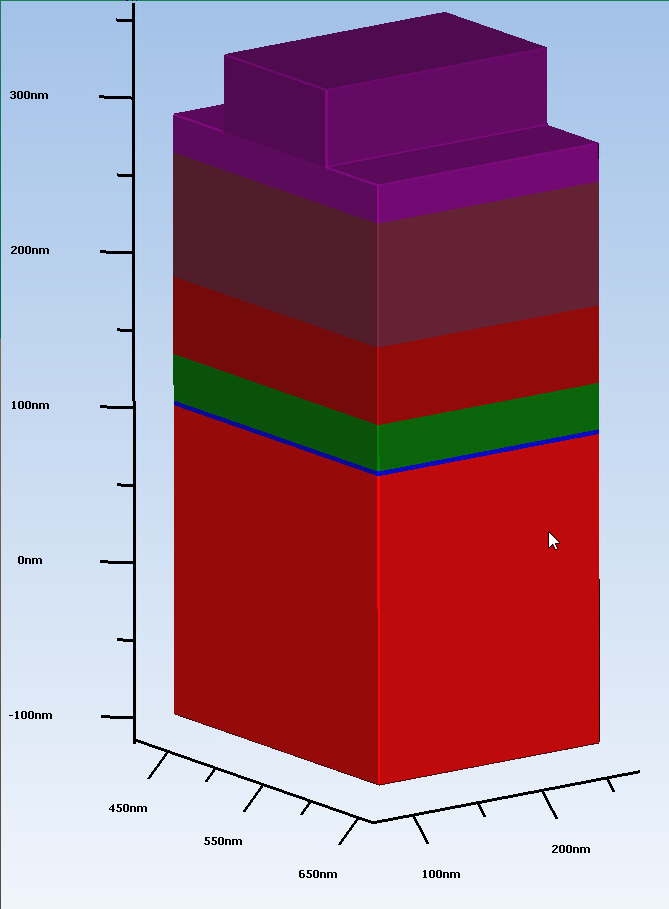
\includegraphics[width=\linewidth]{pics/lth_mand.png}}
\caption{The silicon stack after LTH Mand.}
\label{lth_mand}
\end{figure}

\paragraph{RIE Mand} Reactive ion etching (RIE) \cite{1481759} is used to cut
the SiARC layer, exposing the ODL underneath.

\section{Middle-of-Line}
Explanation on MOL.

\section{Extract Devices}
Explanation on extracting devices.

\section{Conclusion}
Lots of things happen in the 14 nm process flow.

\clearpage
\bibliographystyle{IEEEtran}
\bibliography{bibs}

\end{document}

